\chapter{結論與未來展望}

\section{結語}

\subsubsection{理解遊戲引擎的架構}
透過理解遊戲引擎的架構,能夠知道一個好的遊戲引擎需要甚麼要素,並理解每個元件的原理,藉此從零打造出一個可編輯的遊戲引擎,並透過遊戲引擎加速整體的遊戲開發時程。

\subsubsection{學習遊戲設計模式與理論}
在初期,我們也參考許多的遊戲設計模式,目的是為了增進程式碼的品質並減少程式碼的耦合度,藉此能讓程式之擴充性。

\subsubsection{熟悉語言開發和專案合作工具}
透過GitHub進行程式碼託管,並用Trello進行專案管理,以及利用Slack進行團隊的溝通,便於版本控制以及組員們的溝通和進度檢視。

%%%%%%%%%%%%%%%%%%%%%%%%%%%%%%%%%%%%%%%%%%%%%%%%%%%%%%%%%%%%%%%%%%%%%%%%
\section{實際產出}

\subsubsection{BatchRendering}

在加入 Batch Rendering 後,RishEngine 的 Renderer 獲得了顯著的提升:

\begin{table}[h]
\centering
    \begin{tabular}{@{} *{5}{c} @{}}
    \headercell{Number of \\ Sprites} & \multicolumn{4}{c@{}}{Modes}\\
    \cmidrule(l){2-5}
    & Debug Non-batch & Release Non-batch & Debug Batch & Release Batch    \\ 
    \midrule
    100    & 1000 &  1055   &  1900 &  2789 \\
    1000   & 167  &  158    &  568  &  1379 \\
    10000  & 18   &  17     &  82   &  247  \\
    100000 & < 1    &  < 1  &  9    &  28   \\
    \end{tabular}
\caption{不同 Rendering 方法下 FPS 差別}
\label{tab:abc}
\end{table}

可以發現到:加入 Batch Rendering 後,Renderer 的效率獲得了巨大的提升,在小規模數量的 Sprites 時,FPS 的增加相當可觀;但數量一大起來時,增加的幅度就變小了,由此可知在數量大時渲染瓶頸在其他地方。

\begin{figure}[h]
    \begin{subfigure}{0.5\textwidth}
        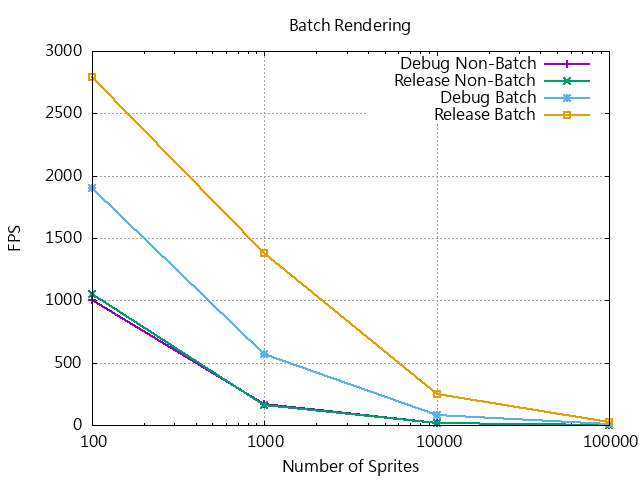
\includegraphics[width=0.9\linewidth, height=5cm]{./resources/batch_compare.png} 
        \caption{不同 Rendering 方法}
        \label{fig:subim1}
    \end{subfigure}
    \begin{subfigure}{0.5\textwidth}
        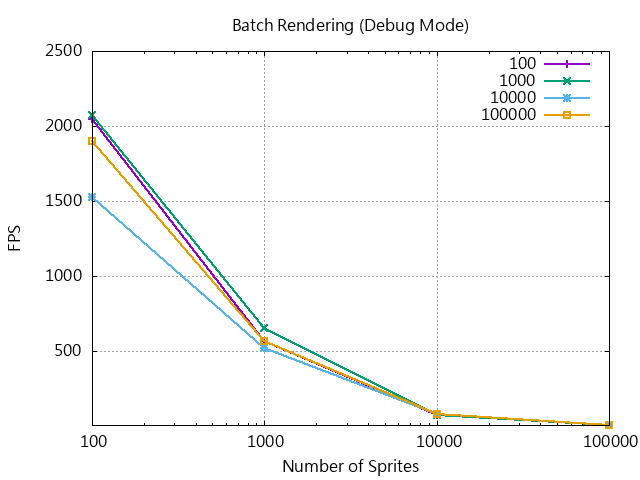
\includegraphics[width=0.9\linewidth, height=5cm]{./resources/max_index.png}
        \caption{不同 Max Index}
        \label{fig:subim2}
    \end{subfigure}
\caption{不同 Rendering 方法效能比較}
\label{fig:image2}
\end{figure}

\subsubsection{Particle System}

目前這個Particle System能夠做出像是煙霧、煙火、火焰、雪等效果,各種其他特效 也能透過條參數來獲得效果,且還能控制排放的間隔,每多少秒才排放一次。未來希 望能夠新增更多的particle排放的曲線,不只能夠調整參數,能夠有個函數圖形讓使用者們直接選取中意的曲線,來模擬particle的路徑。

\subsubsection{2D Lighting}

擁有平面的光源之後,就能夠讓遊戲畫面更加的豐富,我們能夠調動世界的光暗,讓世界是暗的,只有擁有光源的地方能夠產生亮光。

\subsubsection{Physics}

擁有了物理模擬,能夠讓遊戲能夠更趨於真實。雖然我們重造了輪子,市售上的遊戲物理引擎有很多種,但透過本次專案我習得了物理引擎的原理,包括裡面許多一些物理公式的來龍去脈證明,以及為了加速而使用到的演算法優化方法,使整個物理引擎能夠更流暢的運作。

\subsubsection{Editor}
最後,我們利用上述所學的知識和理論,打造出一個能夠撰寫出遊戲之遊戲引擎。使用者只需透過針對物件撰寫腳本,並對於特定的物件撰寫事件觸發的相關邏輯,就能簡易的打造出遊戲。除此之外,也有一些能夠幫助開發者撰寫遊戲的小工具(ex: 拖曳、群組、伸縮物件…等),藉此來加速遊戲開發。

\begin{figure}[h]
    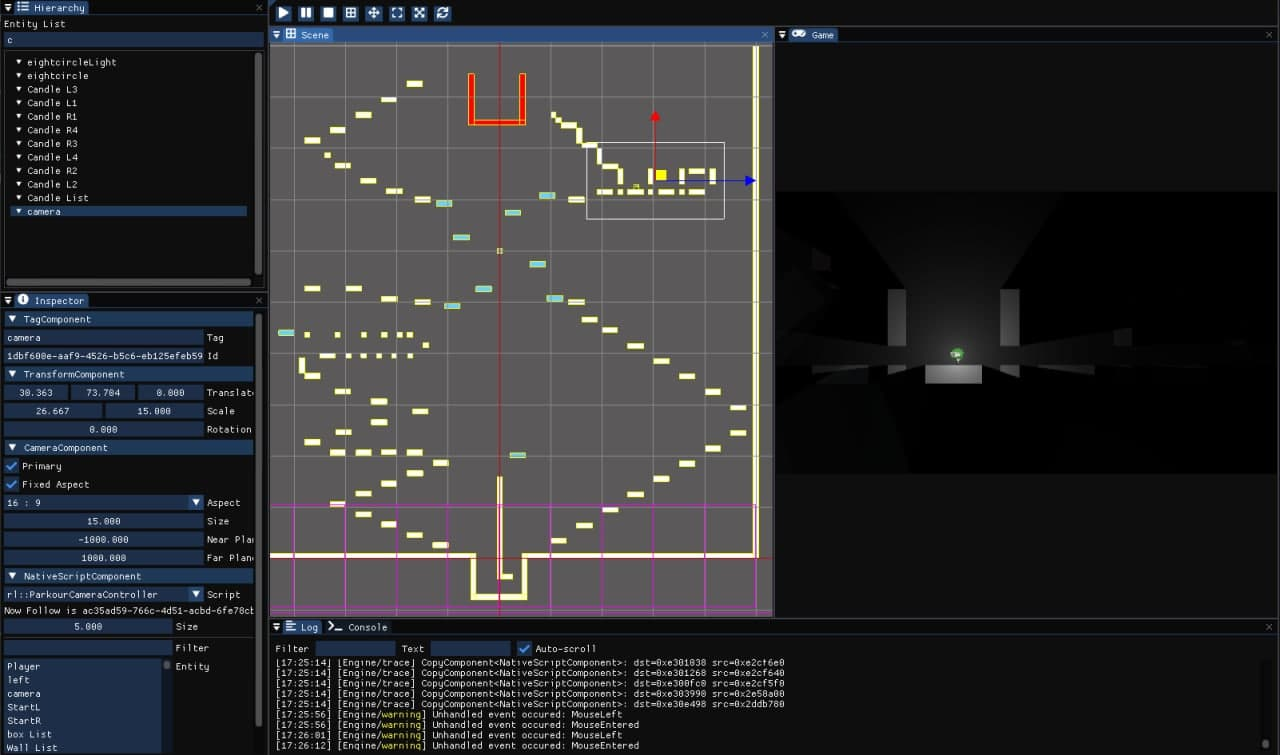
\includegraphics[width=\linewidth]{./resources/gametest.jpg}
\caption{用RishEngine產出遊戲}
\label{fig:gametest} 
\end{figure}

%%%%%%%%%%%%%%%%%%%%%%%%%%%%%%%%%%%%%%%%%%%%%%%%%%%%%%%%%%%%%%%%%%%%%%%%
\section{未來展望}

\subsubsection{Renderer}

\begin{itemize}
\item{將 Renderer 變成 Multi-thread 架構}
    \SubItem{由於 OpenGL 在設計當初並沒有考慮到多線程,因此如果要在 OpenGL 使用多線程架構則要用 C++ 模擬,相較於其他現代的 API ,就沒有此限制(Vulkan, DirectX)。}
    \SubItem{將程式分成 Main Thread 與 Rendering Thread}
        \SubSubItem{Main Thread 主要負責遊戲循環,如果要畫東西時,會將 Render 資訊打包成一個 Task,接著加到共用的 Rendering Queue 中(Message Queue)。}
        \SubSubItem{Rendering Thread 負責消化 Rendering Queue 中的 Task ,向 GPU 發起 Draw Call。}
    \SubItem{在原本單線程的 Renderer 中,主要的瓶頸在 Submit Draw Call,繪製時必須等待繪製好了(Blocking),改成多線程則可以解決這個問題。}
\end{itemize}

\subsubsection{Scripting Languag}

\begin{itemize}
\item{目前 RishEngine 直接使用 C++ 作為 Script 的語言,優點是可以直接使用引擎的 C++ API,但缺點就是編譯非常花時間}
\item{可以使用開源的專案,接著只要提供該語言的引擎 API 之後,便可以用該腳本語言撰寫遊戲邏輯}
    \SubItem{例如 \lstinline{mono(C#)}、\lstinline{sol2(lua)}、\lstinline{pybind11(python)} 綁定腳本語言}
\item{動態語言雖然效能沒有編譯語言好,但動態語言不用等待編譯,這對需要快速迭代的遊戲來說至關重要}
\end{itemize}

\subsubsection{支援3D遊戲設計}
因為專題時程關係,我們為了降低以及加速開發,只針對平面遊戲引擎。希望未來能夠支援3D,讓遊戲引擎支援更多也更豐富。

\newpage